\documentclass[a4paper]{article}
\usepackage[utf8]{inputenc}
\usepackage[margin=0.5in]{geometry}

\usepackage{graphicx}
\pagenumbering{gobble}

\begin{document}

\section*{Appendix}
We put here all the plots used in the report at a bigger scale in the order of apparition of the report. Some plots contain more information that those presented in the report. For instance, figure \ref{timeline_wide_1} contains all the European countries while in the report, there was only a random sample of 14 countries.

\hspace{5cm}

\begin{figure}[h]
   \centering
   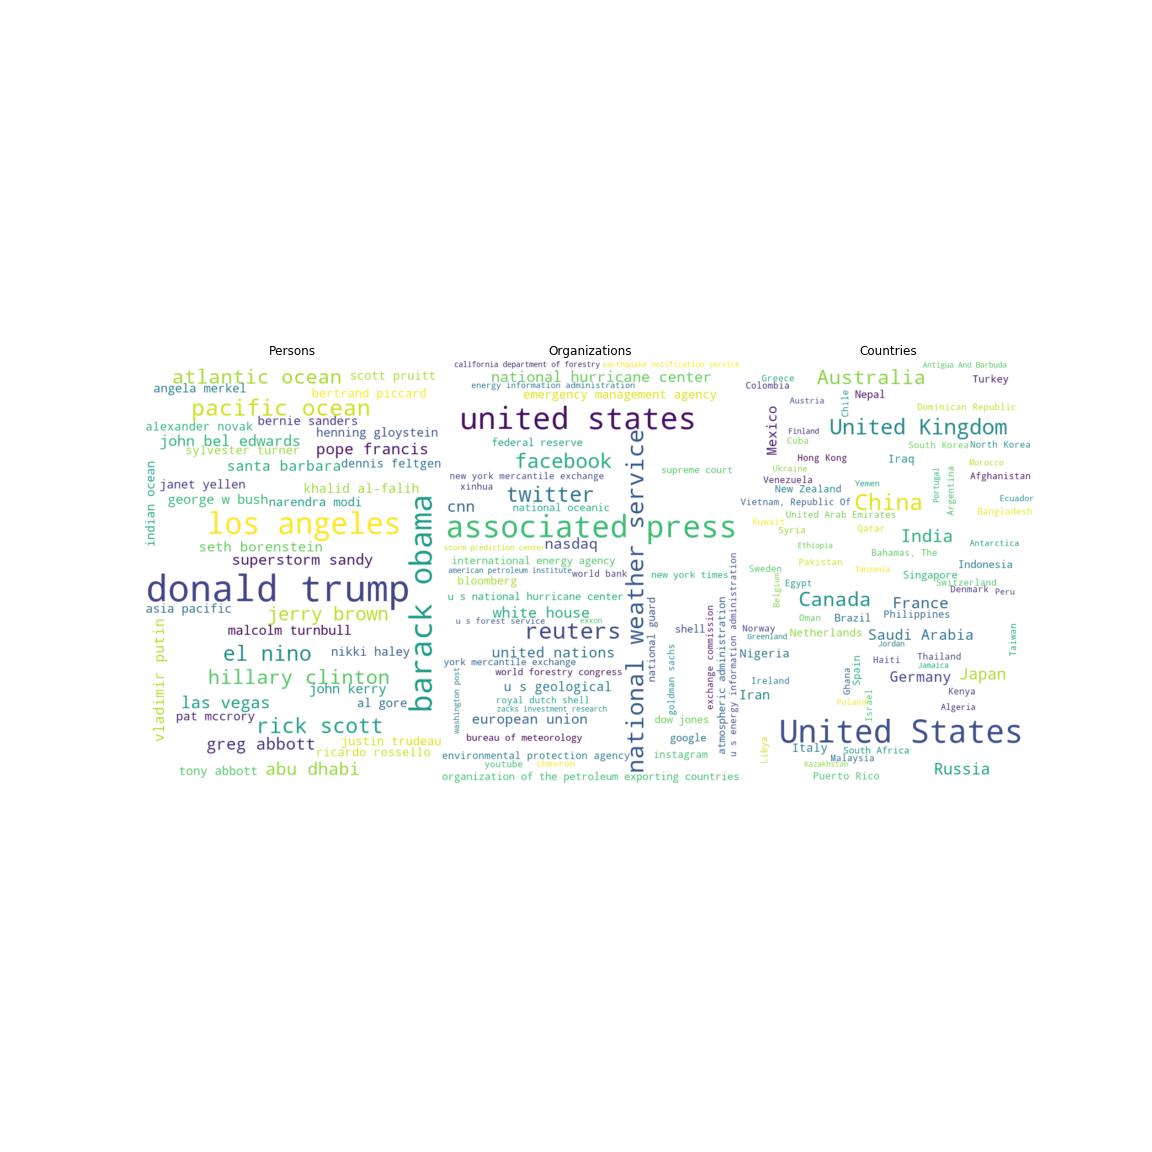
\includegraphics[scale=0.4]{wordcloud_global.png}
   \caption{\label{actors_wide} Word Cloud of most mentioned organizations, persons and locations.}
\end{figure}

\begin{figure}[h]
   \centering
    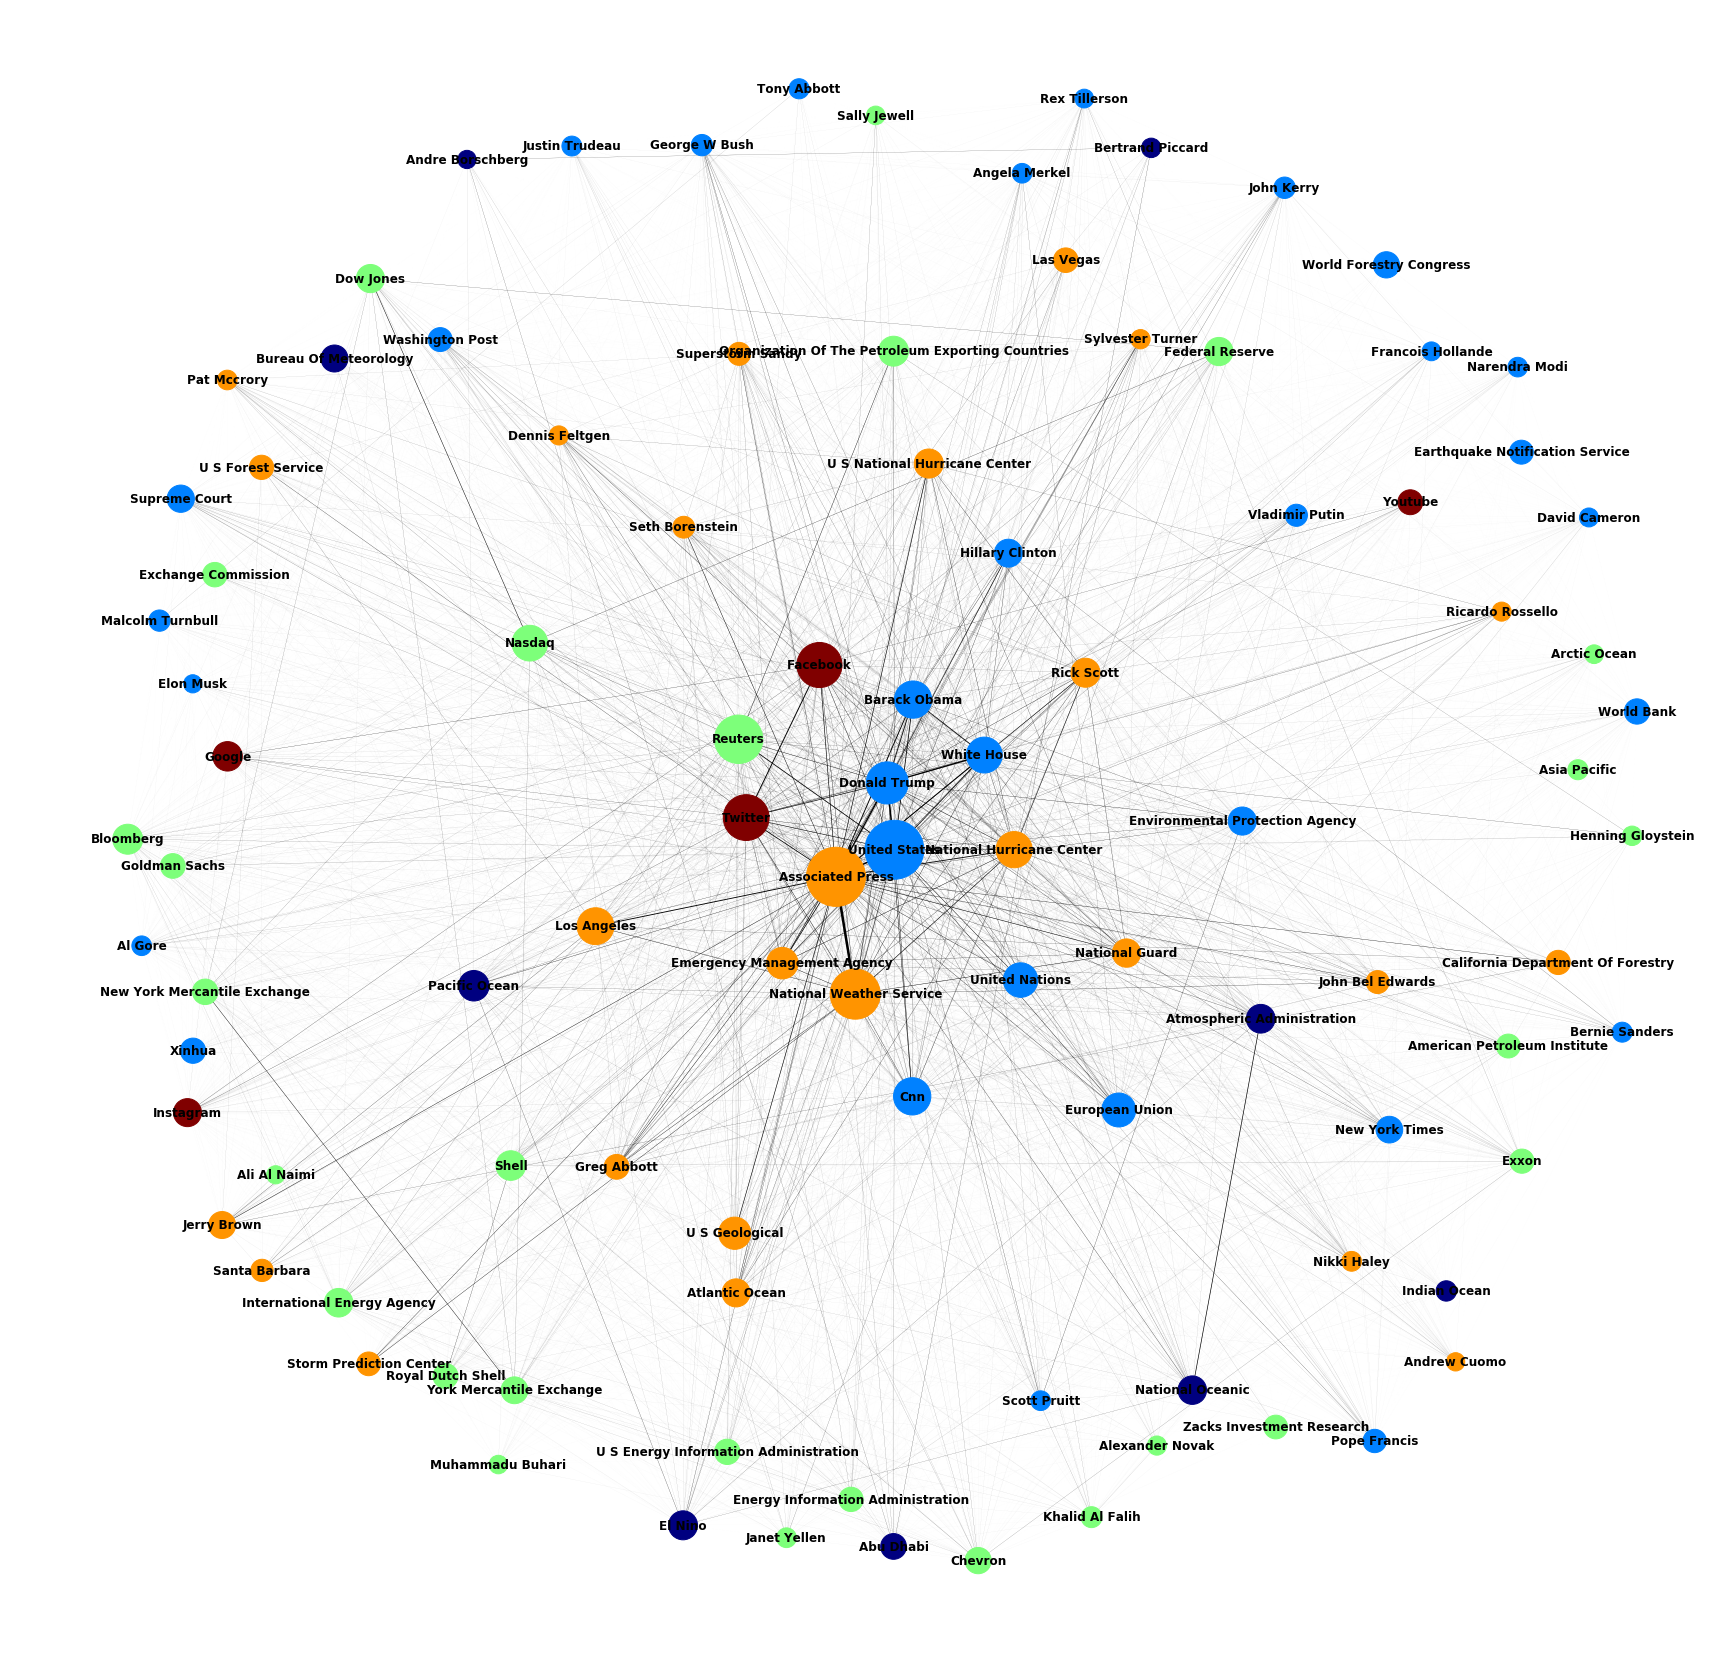
\includegraphics[scale=0.2]{top_50.png}
    \centering
    \caption{\label{network_wide} Co-occurrence network of the top 50 organizations and top 50 persons colored by communities}
\end{figure}
\clearpage

\begin{figure}[h]
   \centering
    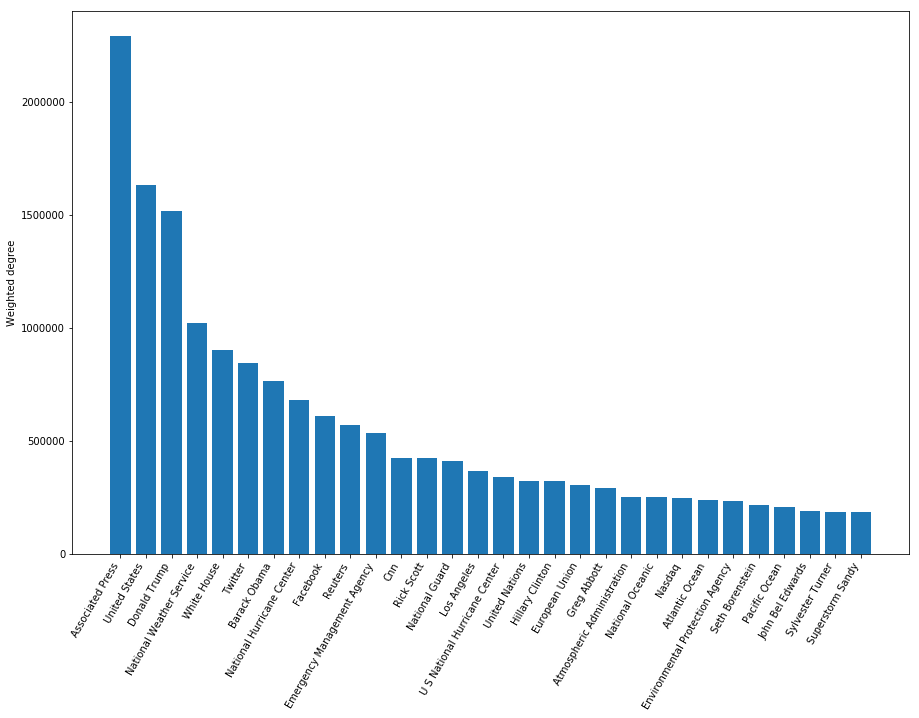
\includegraphics[scale=0.4]{weighted_degree_dist.png}
    \centering
    \caption{\label{weighted_degree} Distribution of the weighted degree between the top 50 organizations and top 50 persons (30 first results)}
\end{figure}

\begin{figure}[h]
   \centering
   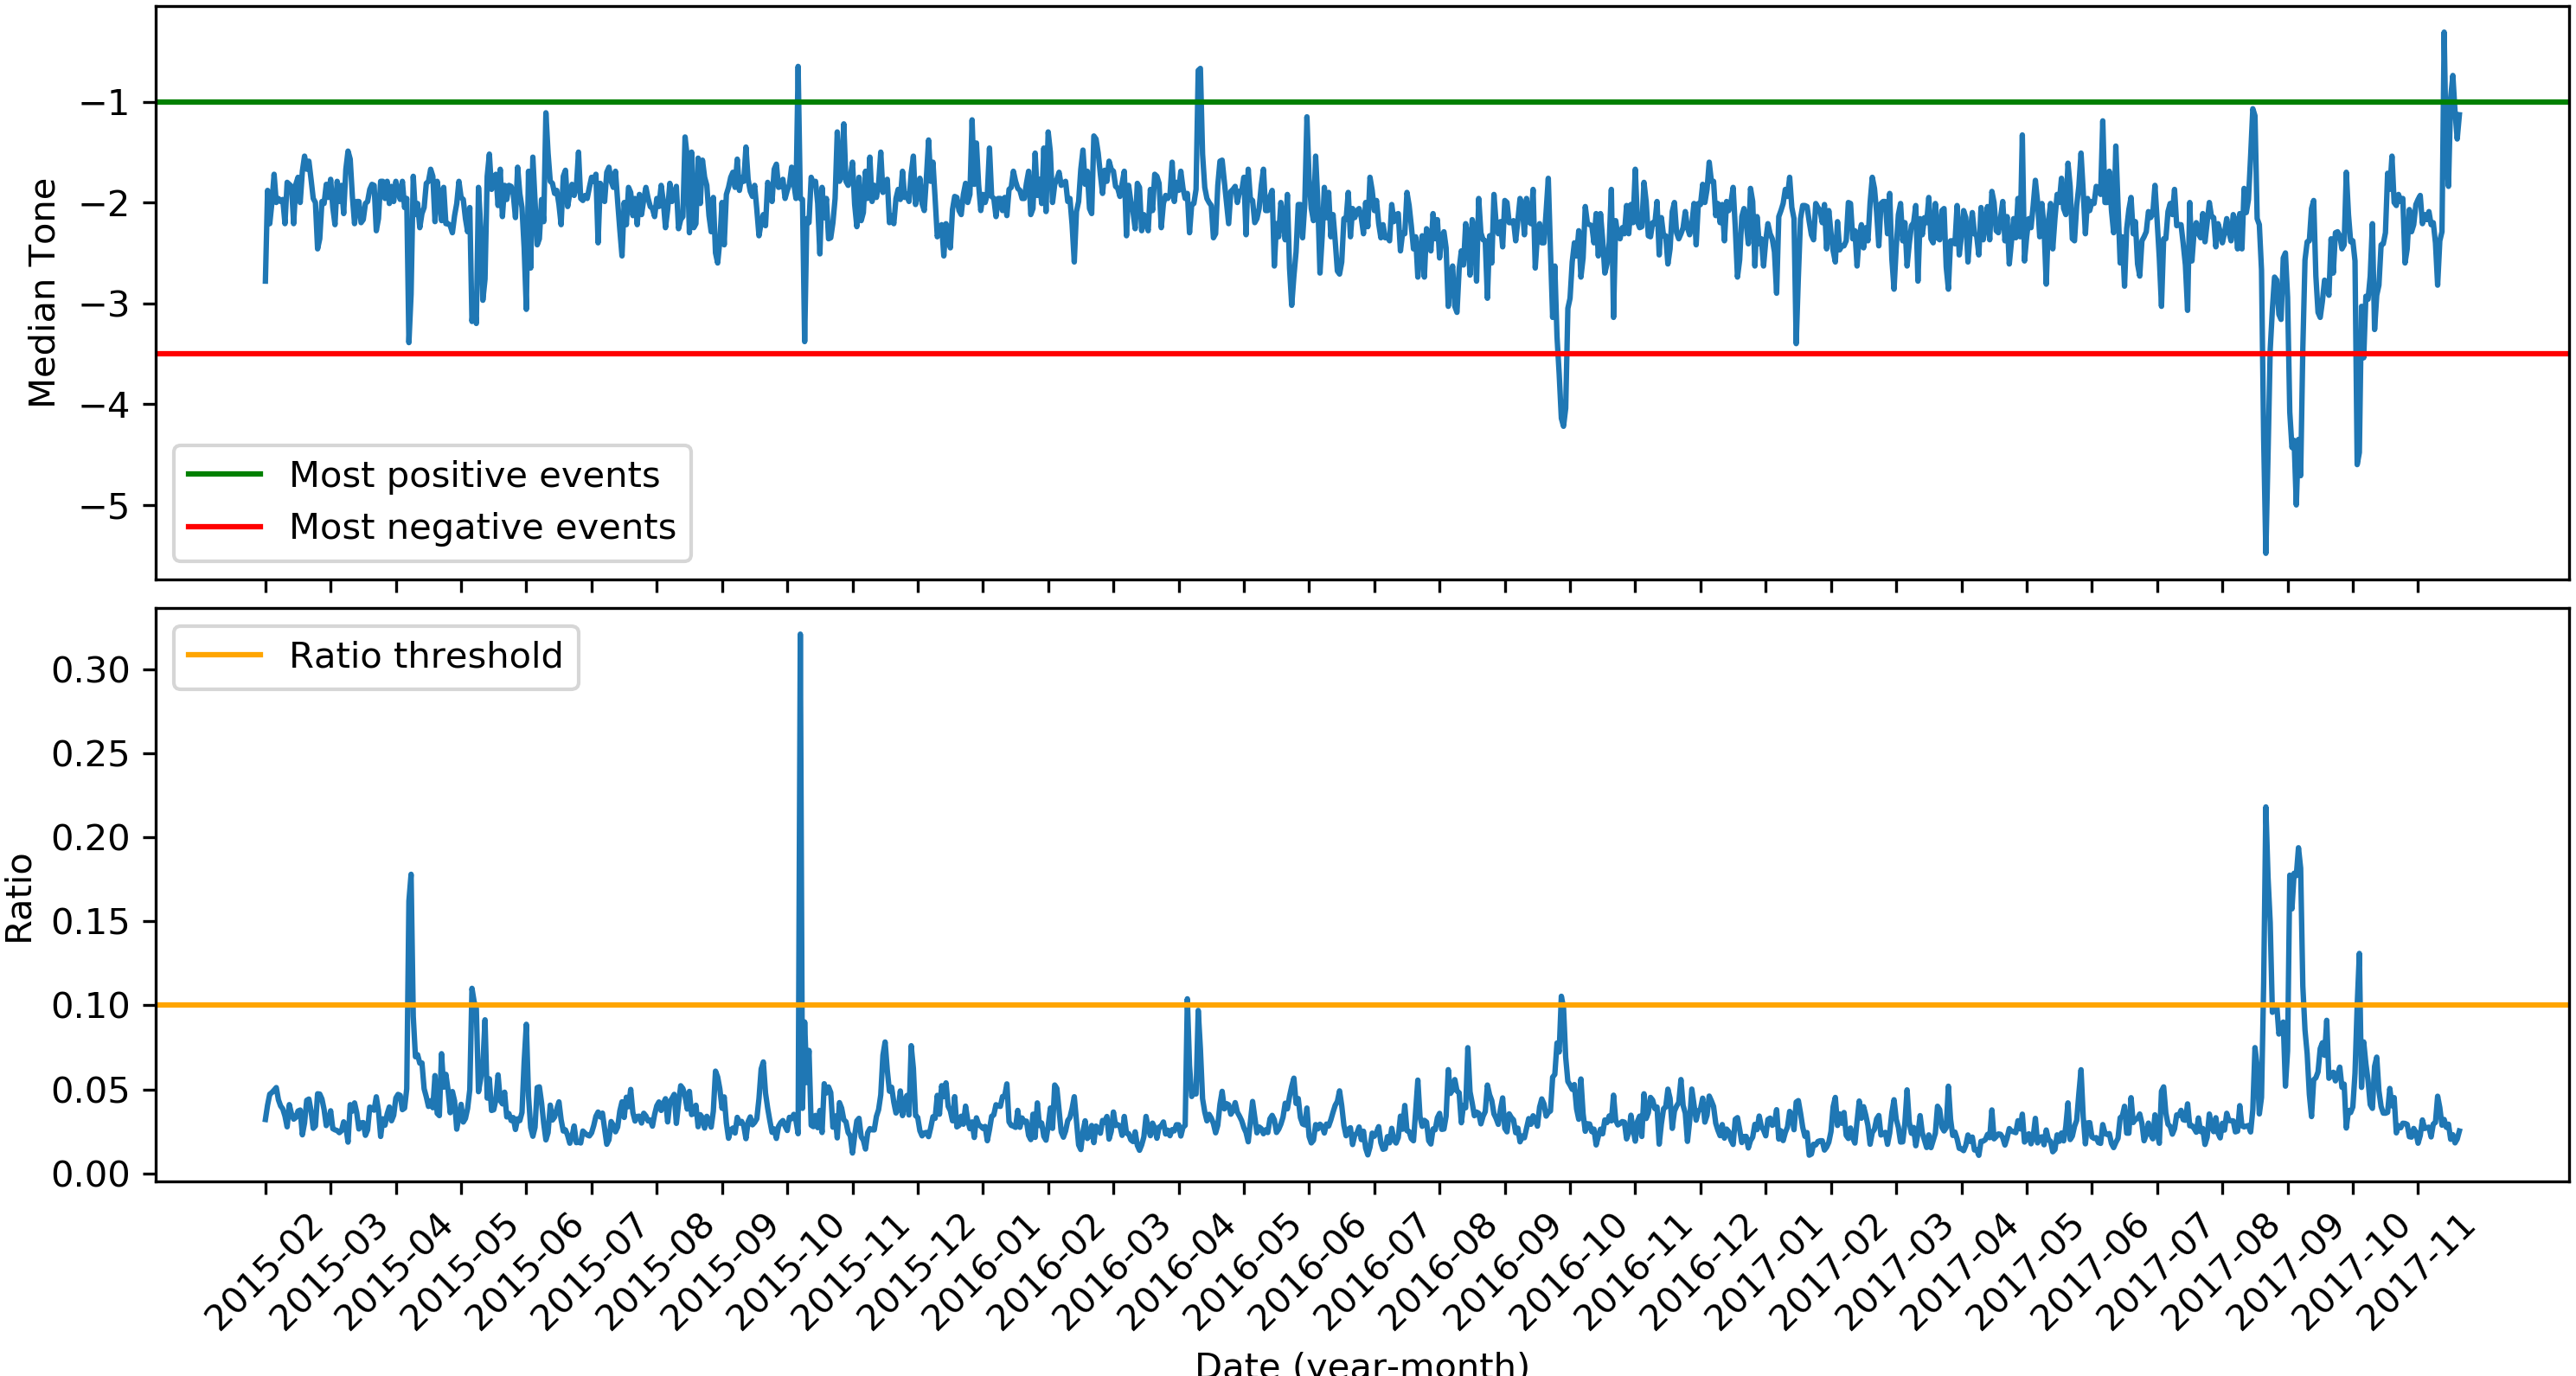
\includegraphics[scale=0.5]{global_ratio_tone_plot.png}
    \caption{\label{time_evolu_wide} Global median mentions ratio (top) and tone (bottom)}
\end{figure}

\begin{figure}[h]
   \centering
   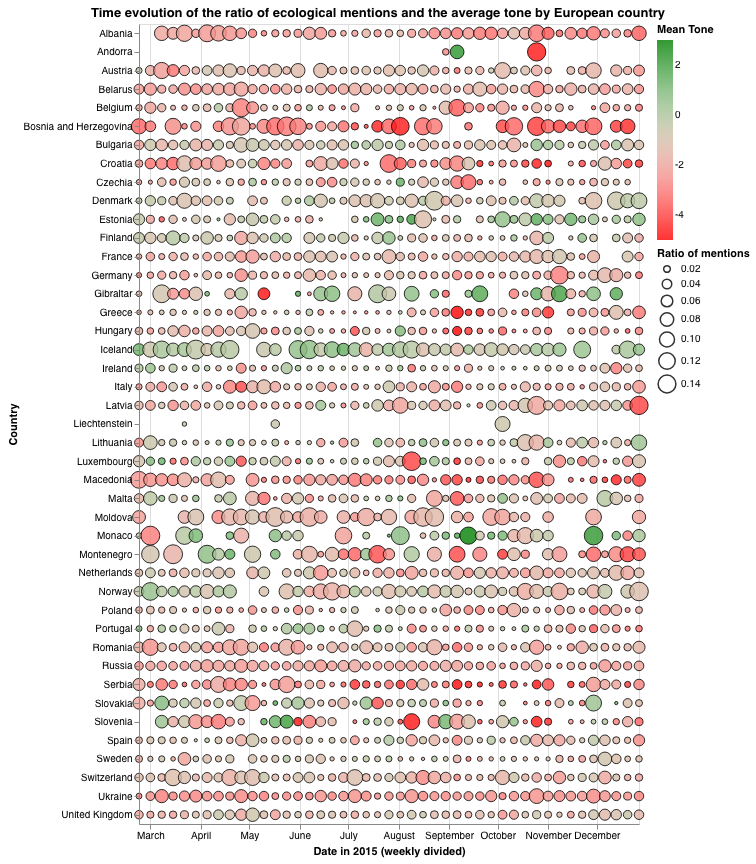
\includegraphics[scale=0.5]{timeline_europe_2015.png}
    \caption{\label{timeline_wide_1} Time evolution of the ratio of mentions and tone in articles mentioning a European country in 2015}
\end{figure}

\begin{figure}[h]
   \centering
   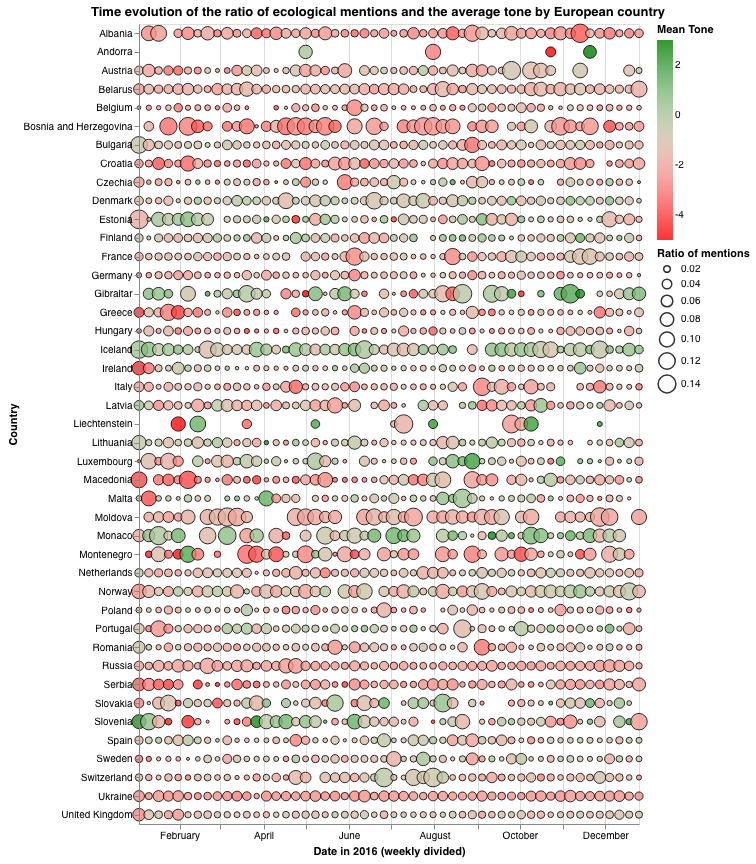
\includegraphics[scale=0.5]{timeline_europe_2016.png}
    \caption{\label{timeline_wide_2} Time evolution of the ratio of mentions and tone in articles mentioning a European country in 2016}
\end{figure}

\begin{figure}[h]
   \centering
   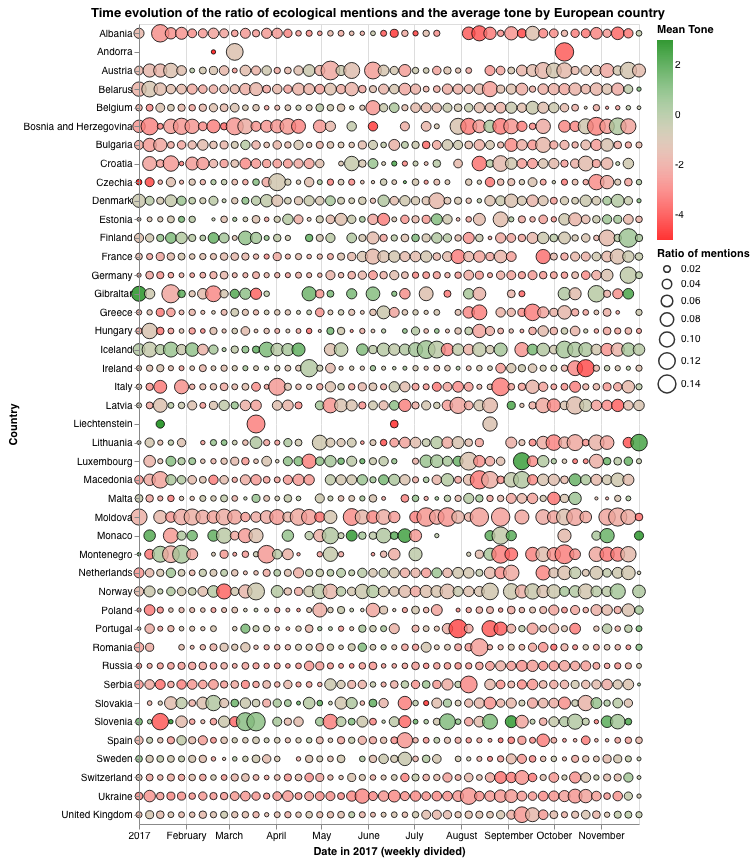
\includegraphics[scale=0.5]{timeline_europe_2017.png}
    \caption{\label{timeline_wide_3} Time evolution of the ratio of mentions and tone in articles mentioning a European country in 2017}
\end{figure}

\begin{figure}[h]
   \centering
   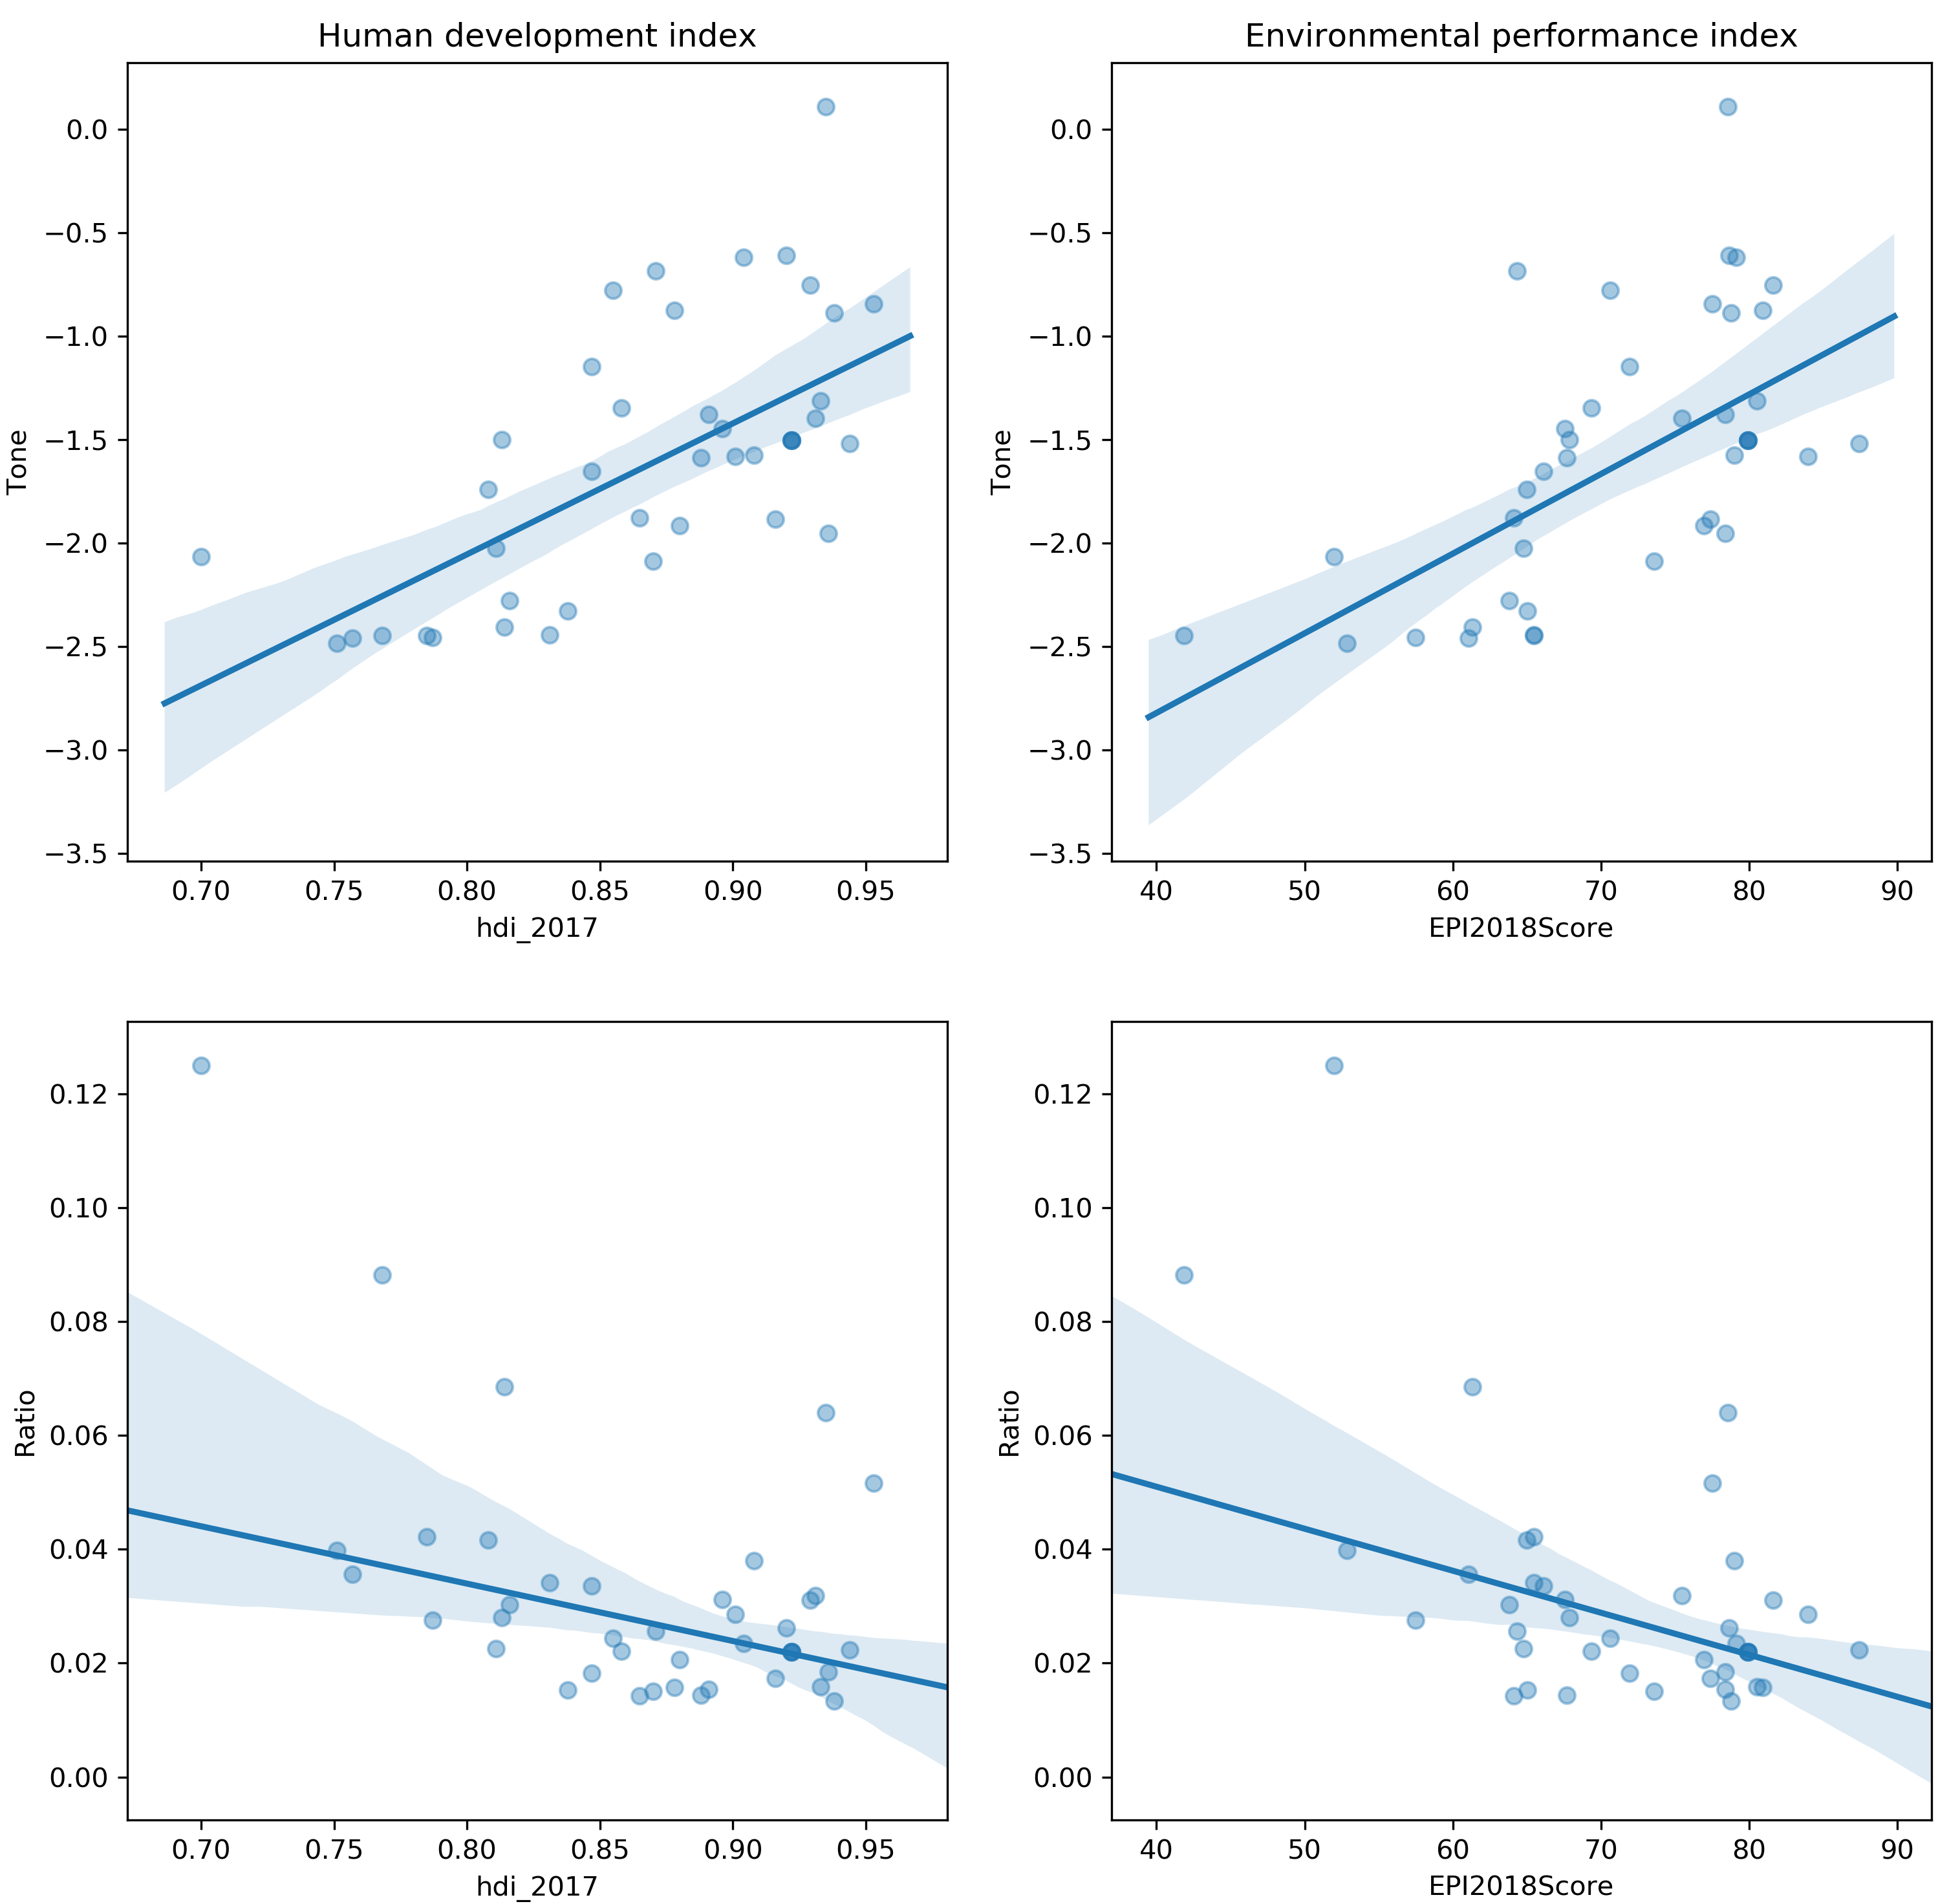
\includegraphics[scale=0.5]{corre_europe.png}
    \caption{\label{corre_wide} Correlation of the tone and the ratio of mentions in articles mentioning any European country with the Human development index and the Environmental performance index}
\end{figure}


\begin{figure}[h]
   \centering
   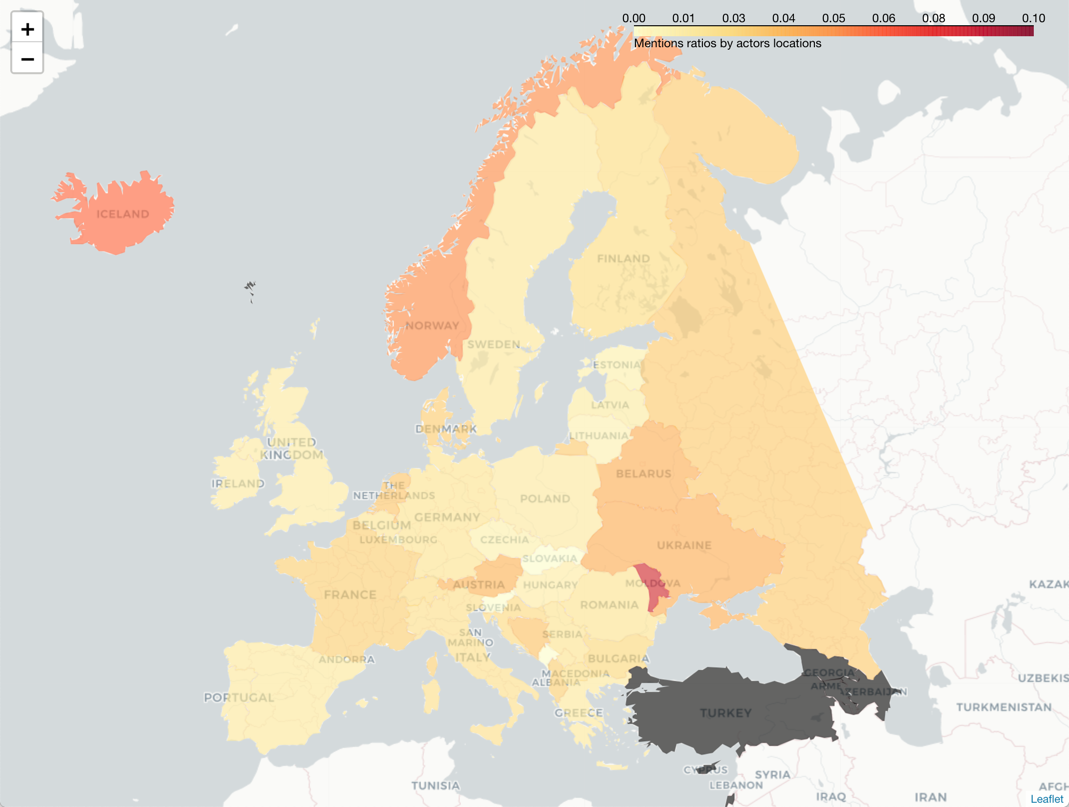
\includegraphics[scale=0.5]{map_europe_actors.png}
    \caption{\label{corre_wide} Ratio of mentions in articles mentioning European countries}
\end{figure}

\begin{figure}[h]
   \centering
   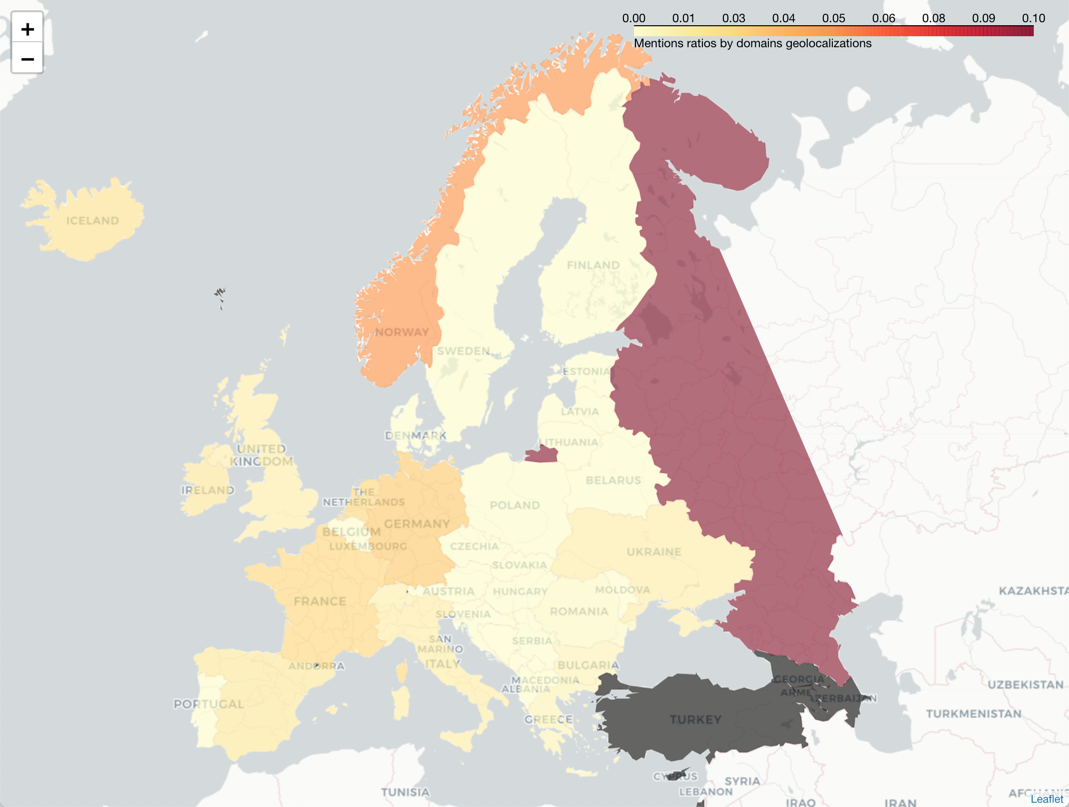
\includegraphics[scale=0.5]{map_europe_domains.png}
    \caption{\label{corre_wide} Ratio of mentions in articles by media hosted by European countries}
\end{figure}

\end{document}
